\newpage
\begin{flushleft}
  \textbf{\large 3 Разработка системы для проведения экспериментальных исследований }
\end{flushleft}
\refstepcounter{chapter}
\addcontentsline{toc}{chapter}{3 Разработка системы для проведения экспериментальных исследований}
В данной главе будут рассмотрены выбранные для системы апробирования компоненты и описан процесс их подготовки.

\section{Выбор микрокомпьютера}
На данный момент на рынке представлено множество микрокомпьютеров. Наиболее распространенными из них являются Orange Pi, Nvidia Jetson и Raspberry Pi. 

Идеальным выбором для запуска тяжеловесных алгоритмов является Nvidia Jetson, но он обладает рядом недостатков:
\begin{itemize}
  \item высокая цена;
  \item высокое энергопотребление;
  \item относительно низкая распространенность в России;
  \item большой вес у старших моделей.
\end{itemize}

Перечисленные недостатки критичны, особенно в задачах мобильной робототехники, где энергоэффективность и рабочий вес наиболее чувствительные параметры. 
Orange Pi является подобием Raspberry Pi, но при этом обладает худшей поддержкой и меньшей распространенностью. 

Raspberry Pi является идеальным выбором в силу следующих причин:
\begin{itemize}
  \item низкая цена -- в России можно найти предложения за 10000 рублей;
  \item малый вес -- плата весит 50г;
  \item высокая энергоэффективность;
  \item доступность в России;
  \item отличная поддержка;
  \item большое количество информации в интернете;
  \item внешние вычислительные модули TPU, разработанные специально для платформы. 
\end{itemize}

Именно поэтому для стенда апробации был выбран микрокомпьютер Raspberry PI 5 8GB.

\section{Выбор дополнительного вычислительного модуля}
В качестве дополнительного вычислительного модуля в работе будет использоваться TPU (англ. Tensor Processing Unit -- устройство обработки тензоров). Использование TPU позволяет оптимизировать работу с тензорами с помощью параллельных вычислений.
Благодаря этому, скорость работы нейронных сетей возрастает в разы. На данный момент на рынке РФ представлены TPU двух компаний: Google Coral и Hailo. 

Hailo является более новой разработкой, мощнее и эффективнее. Однако, в связи с его новизной, все еще остаются проблемы и баги, которые могут быть критичны при использовании. Также сама процесс взаимодействия с Hailo требует переписывания всего кода, так как требует использования отдельной библиотеки. 

В свою очередь Google Coral требует только конвертировать веса нейронной сети в специальный формат, после чего все происходит в автоматическом режиме. Для его работы не требуется переписывать ни единой строчки кода. 
Также существуют различные версии, которые позволяют подключение с использованием различных портов: M2, Mini PCIe, USB. 
Существует еще и версия с двумя ядрами, что дает возможность одновременно запускать две разных нейронных сети независимо друг от друга. 

По совокупности удобства использования, доступности и проверенной временем надежности выбор пал на внешний вычислительный модуль Google Coral M.2 Accelerator with Dual Edge TPU и плата для подключения Pineboards AI Dual. 

\section{Настройка и подключение компонентов}
Для удобства работы была выбрана операционная система Raspberry PI OS, так как она сразу включает в себя все нужные драйвера для Raspberry Pi, а также удобный интерфейс для их настройки. 
Дополнительно нужно только поставить драйвера Google Coral, представленные на официальном сайте Google Coral. 

\section{Функциональная схема системы}

Итоговая функциональная схема системы представлена на рисунке \ref{fig:func_scheme}. 
\begin{figure}[ht]
  \centering
  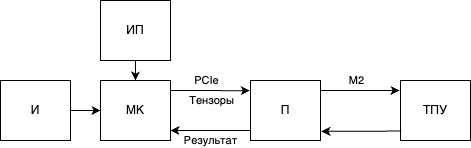
\includegraphics[width=\textwidth]{schemes/func.drawio.png}
  \caption{Функциональная схема системы: И -- изображение; ИП -- источник питания; МК -- микрокомпьютер Raspberry PI 5; П -- плата Pineboards AI Dual; ТПУ -- Google Coral TPU Dual;}
  \label{fig:func_scheme}
\end{figure}
При тестировании алгоритмов на вход микрокомпьютера будет подаваться изображение. После первичной обработки оно посредством платы передается на TPU для проведения вычисления нейронной сети детектора, после чего результат возвращается обратно на микрокомпьютер для последующей обработки алгоритмом отслеживания.
\section{Выводы по главе}
В главе были разобраны представленные на рынке варианты микрокомпьютеров и вычислительных модулей TPU. В итоге выбраны комплектующие для стенда апробации:
\begin{itemize}
  \item микрокомпьютер -- Raspberry Pi 5 8GB.
  \item вычислительный модуль -- Google Coral TPU Dual;
  \item плата для подключения -- Pineboards AI Dual.
\end{itemize}
% TODO: CHECK WEIGHT 
Общая стоимость компонент составляет 28000 рублей; масса -- 100г. 